% reports/report_latex/main.tex
% Book Rating Prediction – Final Academic Report
% Authors: Nahasat Nibir, Jett Guitteau, Sébastien Martel, & Sunny Mondal
% Date: Summer 2026
\documentclass[11pt,a4paper]{article}
\usepackage[utf8]{inputenc}
\usepackage[T1]{fontenc}
\usepackage{graphicx}
\usepackage{booktabs}
\usepackage{hyperref}
\usepackage{geometry}
\geometry{margin=1in}
\usepackage{float}
\usepackage{caption}
\usepackage{parskip}
\usepackage{amsmath}

\title{\textbf{Predicting Book Ratings: An End-to-End Machine Learning Pipeline}}
\author{Nahasat Nibir, Jett Guitteau, Sébastien Martel, & Sunny Mondal \\ DSTI School of Engineering / Python Machine Learning Labs}
\url{https://github.com/jettguitteau/book_classification_pythonML}
\date{May-August 2026}

\begin{document}
\maketitle

%---------------------------------------------------------------------
\section{Introduction}
The goal of this project is to build a machine learning model that predicts the average rating of a book (on a 1–5 scale) based on its metadata, such as title, authors, page count, publisher, language, and engagement metrics (ratings count, reviews count). The dataset contains 11,128 books with 12 attributes. After cleaning and feature engineering, we trained and compared multiple regression models, ultimately deploying the best one as a Streamlit web application.

This report details the full pipeline: exploratory data analysis, data cleaning, feature engineering, model selection and evaluation, and deployment.

%---------------------------------------------------------------------
\section{Methodology}

\subsection{Exploratory Data Analysis}
The raw dataset (11,128 rows) was examined for distributions, missing values, and anomalies.
- The target variable \texttt{average\_rating} exhibited a left‑skewed distribution with a mean of approximately 4.0.
- \texttt{num\_pages}, \texttt{ratings\_count}, and \texttt{text\_reviews\_count} all showed heavy right‑skewness, requiring log‑transformation.
- Several date formats were present in \\ \texttt{publication\_date}, and language codes included variants (e.g., \texttt{en-US}, \texttt{eng}).
- The \texttt{authors} field contained multiple authors separated by “/”.

Figure~\ref{fig:corr_heatmap} shows the correlation matrix of numeric features before cleaning. Outliers were detected via the IQR method and capped at the 99th percentile.

\begin{figure}[H]
\centering
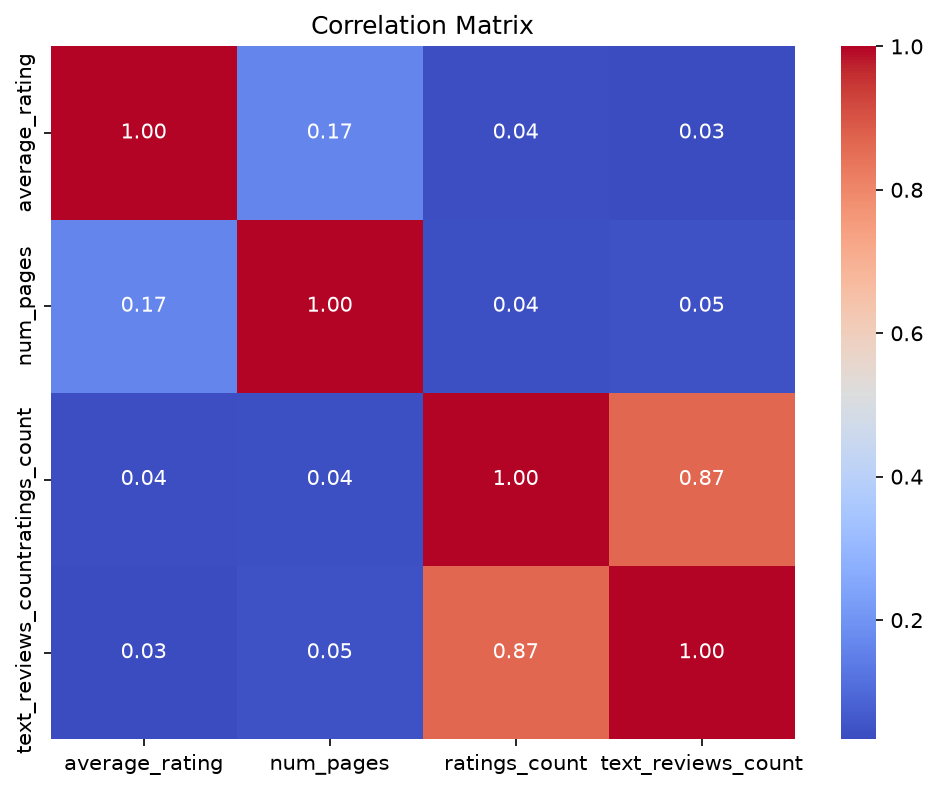
\includegraphics[width=0.7\textwidth]{figures/correlation_heatmap.png}
\caption{Correlation matrix of original numeric features.}
\label{fig:corr_heatmap}
\end{figure}

\subsection{Data Cleaning}
The following cleaning steps were applied:
\begin{itemize}
    \item Parsed \texttt{publication\_date} with \texttt{pd.to\_datetime} (coercing errors); 2 rows with unparseable dates were dropped.
    \item Standardised language codes to ISO 639‑2 (e.g., \texttt{en-US} $\rightarrow$ \texttt{eng}).
    \item Split \texttt{authors} on “/” and created \texttt{author\_count} and \texttt{primary\_author} features.
    \item Limited \texttt{num\_pages} to remain between the 1st and 99th percentile (3-1174.7) to reduce the influence of extreme outliers.
    \item Dropped rows with missing \texttt{average\_rating}.
\end{itemize}
After cleaning, the dataset contained 10,729 books.

\subsection{Feature Engineering}
From the cleaned data, we engineered the following features:
\begin{itemize}
    \item \texttt{title\_length}, \texttt{title\_word\_count}, \texttt{has\_exclamation} (from \texttt{title}).
    \item \texttt{publication\_year}, \texttt{book\_age} (relative to 2026), \texttt{is\_classic} (age > 50).
    \item \texttt{log\_ratings\_count}, \texttt{log\_text\_reviews\_count}, \texttt{reviews\_per\_rating}.
    \item Smoothed target encoding for high‑cardinality categoricals: \texttt{publisher\_te}, \\ \texttt{primary\_author\_te}, \texttt{language\_code\_te}.
\end{itemize}
Identifiers (\texttt{bookID}, \texttt{isbn}, \texttt{isbn13}) and raw text (\texttt{title}) were dropped.

\subsection{Feature Selection}
Mutual information regression and Recursive Feature Elimination (RFE) with a Ridge estimator were used to select the most predictive features. The final set of 8 features was:
\texttt{num\_pages, log\_ratings\_count, log\_text\_reviews\_count, \\ title\_length, publication\_year, publisher\_te, primary\_author\_te}.

\subsection{Model Selection and Comparison}
We trained and compared:
\begin{itemize}
    \item Baselines: Dummy Regressor, Linear Regression, Ridge, Lasso.
    \item Advanced models: Random Forest, XGBoost, LightGBM, CatBoost.
\end{itemize}
All models were evaluated using 5‑fold cross‑validation (RMSE) and a hold‑out test set (80/20 split, random state 42). Hyperparameter tuning was performed with \texttt{RandomizedSearchCV} (20 iterations per model).

%---------------------------------------------------------------------
\section{Results}

\subsection{Model Performance}
Table~\ref{tab:model_comparison} summarises the performance of all models.

\begin{table}[H]
\centering
\caption{Model performance comparison (test set and CV).}
\label{tab:model_comparison}
\begin{tabular}{lccc}
\toprule
\textbf{Model} & \textbf{CV RMSE} & \textbf{Test RMSE} & \textbf{Test R\textsuperscript{2}} \\
\midrule
Dummy Regressor   & 0.2920 & 0.2974 & -0.0002 \\
Linear Regression & 0.2395 & 0.2485 & 0.3018 \\
Ridge             & 0.2395 & 0.2485 & 0.3018 \\
Lasso             & 0.2920 & 0.2974 & -0.0002 \\
Random Forest     & 0.2402 & 0.2461 & 0.3152 \\
LightGBM          & 0.2400 & 0.2446 & 0.3236 \\
CatBoost          & 0.2392 & 0.2450 & 0.3210 \\
\textbf{XGBoost}           & 0.2405 & \textbf{0.2436} & \textbf{0.3292} \\
Ensemble (RF+LGBM) & – & 0.2444 & 0.3245 \\
\bottomrule
\end{tabular}
\end{table}

The XGBoost model achieved the lowest test RMSE (0.2436) and was selected as the final model.

\subsection{Residual Analysis}
Figure~\ref{fig:residual} shows the residual plot for the ensemble model. The errors are roughly symmetrically distributed around zero, with a slight tendency to underpredict very high ratings (\(>4.5\)) and overpredict low ratings (\(<3.0\)), which is expected given the limited representation of extreme ratings in the dataset.

\begin{figure}[H]
\centering
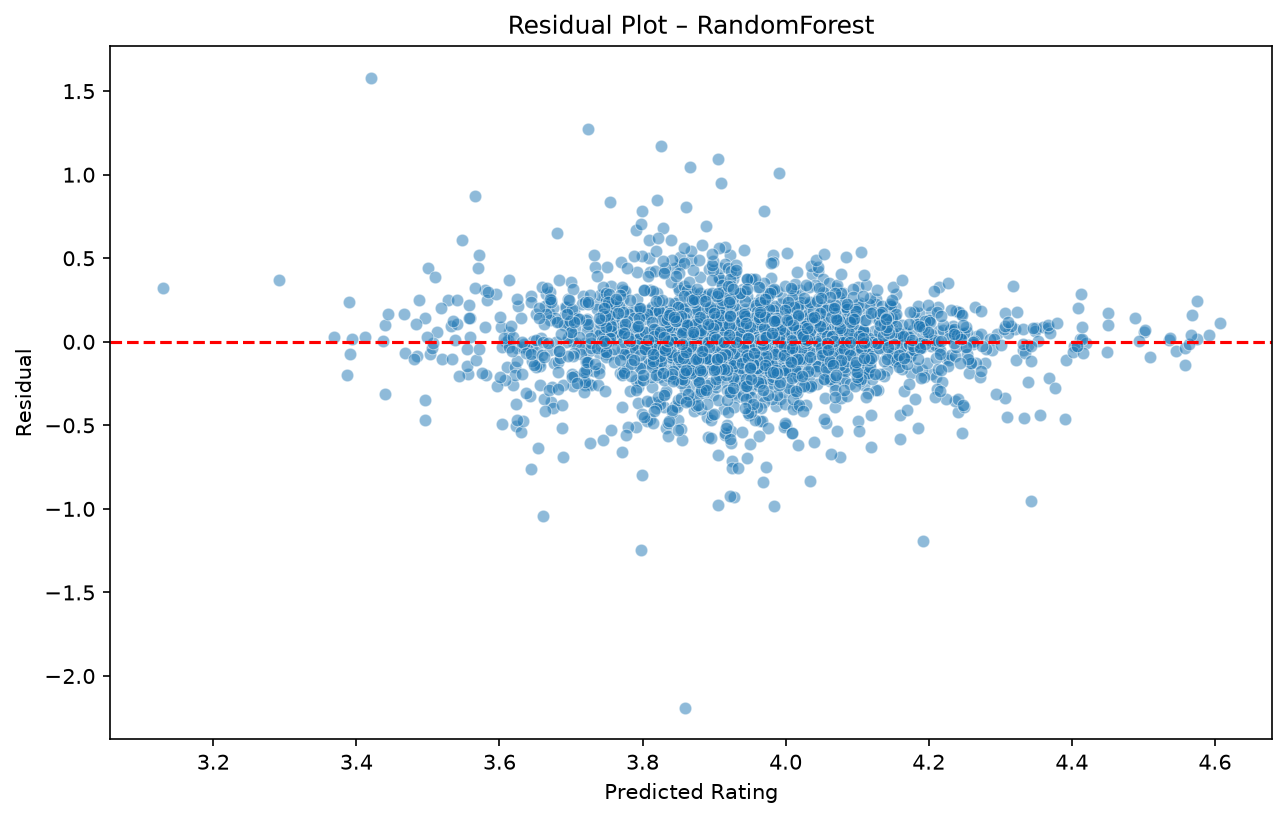
\includegraphics[width=0.65\textwidth]{figures/RandomForest_residual.png}
\caption{Residual plot for the Random Forest model (similar to ensemble).}
\label{fig:residual}
\end{figure}

\subsection{Feature Importance}
Figure~\ref{fig:importance} displays the feature importances from the Random Forest model. The target‑encoded author feature (\texttt{primary\_author\_te}) is by far the strongest predictor, followed by the raw engagement counts. This indicates that the author's historical average rating and the popularity of the book strongly influence its rating – a plausible pattern, though \texttt{ratings\_count} and \texttt{text\_reviews\_count} are post‑publication features and constitute a form of target leakage if we were to predict ratings before the book accumulates reviews. This is discussed further in the Conclusion.

\begin{figure}[H]
\centering
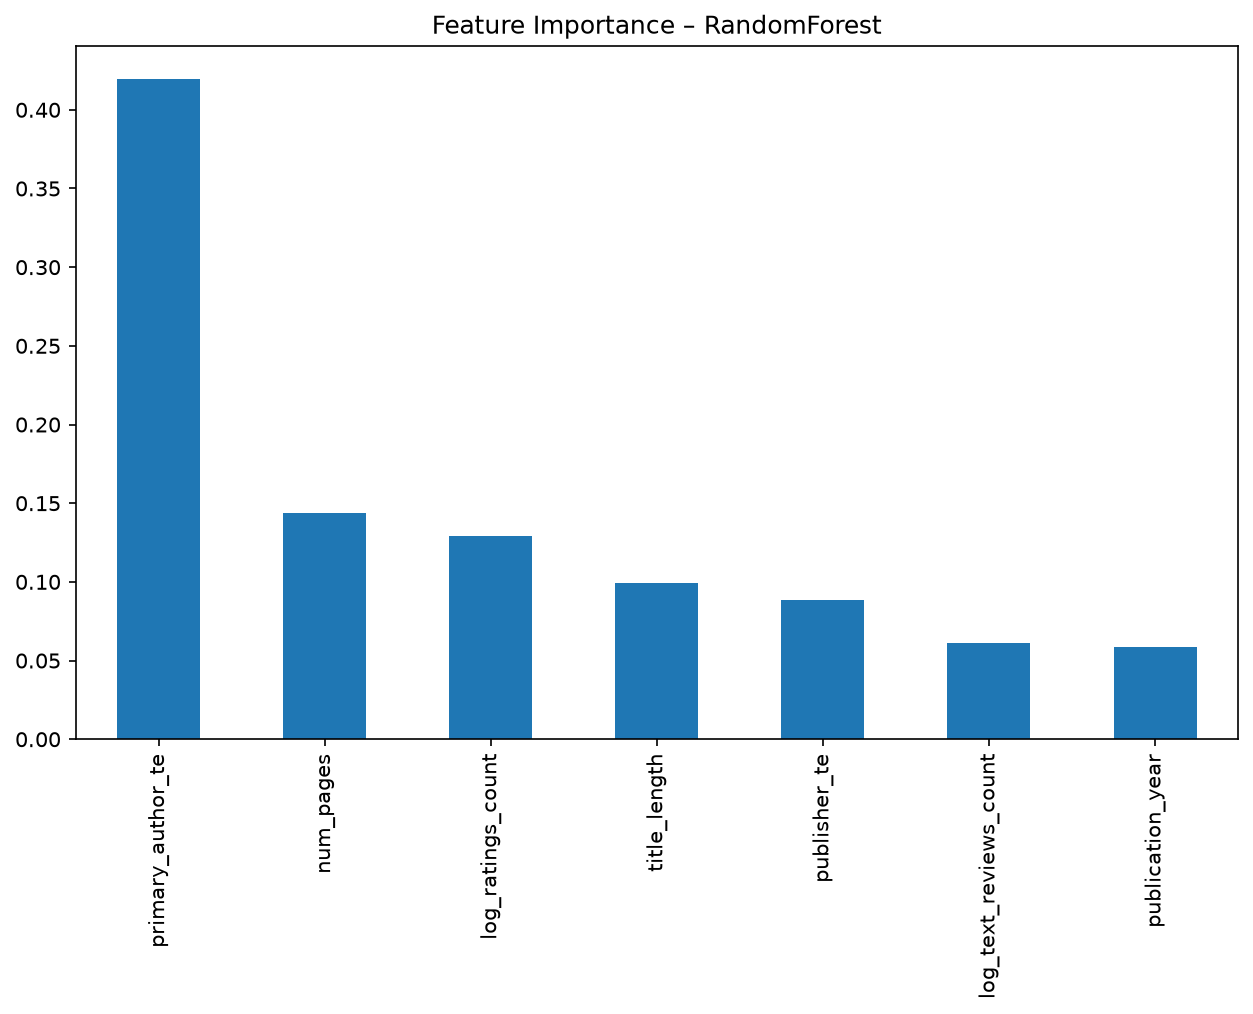
\includegraphics[width=0.75\textwidth]{figures/RandomForest_importance.png}
\caption{Feature importances from Random Forest.}
\label{fig:importance}
\end{figure}

\subsection{Interpretability with SHAP}
SHAP summary plots (not shown due to space) confirmed that \texttt{primary\_author\_te} and \\ \texttt{publisher\_te} have the largest impact on predictions, with higher author/publisher mean ratings pushing the prediction upward. \texttt{log\_ratings\_count} and \texttt{num\_pages} also show positive effects, while \texttt{reviews\_per\_rating} has a mixed influence.

\subsection{Error by Rating Band}
Figure~\ref{fig:error_band} shows that the model performs best on books rated 4–5 (RMSE $\approx$ 0.22) and worst on books rated below 3 (RMSE $\approx$ 0.45). This is partly due to class imbalance: the majority of books in the dataset are highly rated.

\begin{figure}[H]
\centering
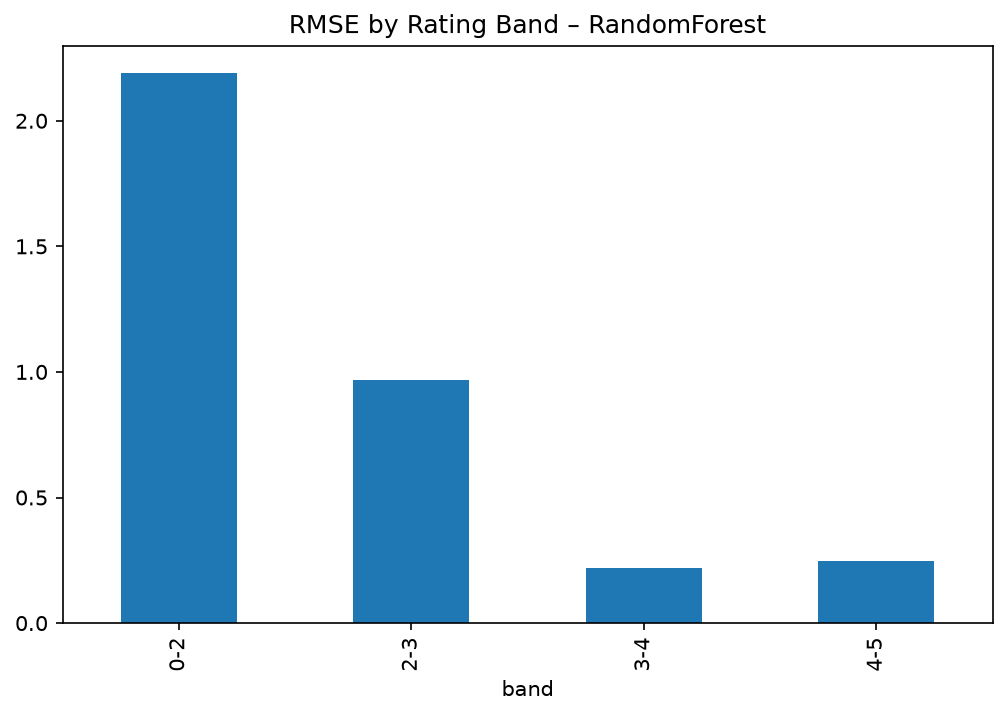
\includegraphics[width=0.65\textwidth]{figures/RandomForest_error_band.png}
\caption{RMSE by rating band.}
\label{fig:error_band}
\end{figure}

%---------------------------------------------------------------------
\section{Deployment}
A Streamlit web application was built to serve the final model. The user interface offers two modes:
\begin{itemize}
    \item \textbf{Single Book}: a form with all required fields (title, authors, pages, ratings count, etc.). After submission, the predicted rating is displayed on a styled card.
    \item \textbf{Batch CSV Upload}: users upload a CSV file with columns similar to the original dataset. The app validates the schema, runs predictions on all rows, and provides a downloadable CSV with an additional \texttt{predicted\_rating} column.
\end{itemize}
The app loads the full preprocessing + model pipeline from a single serialised file \\ (\texttt{best\_pipeline.joblib}), ensuring exact reproduction of the training‑time transformations. The architecture is summarised in Figure~\ref{fig:arch}.

\begin{figure}[H]
\centering
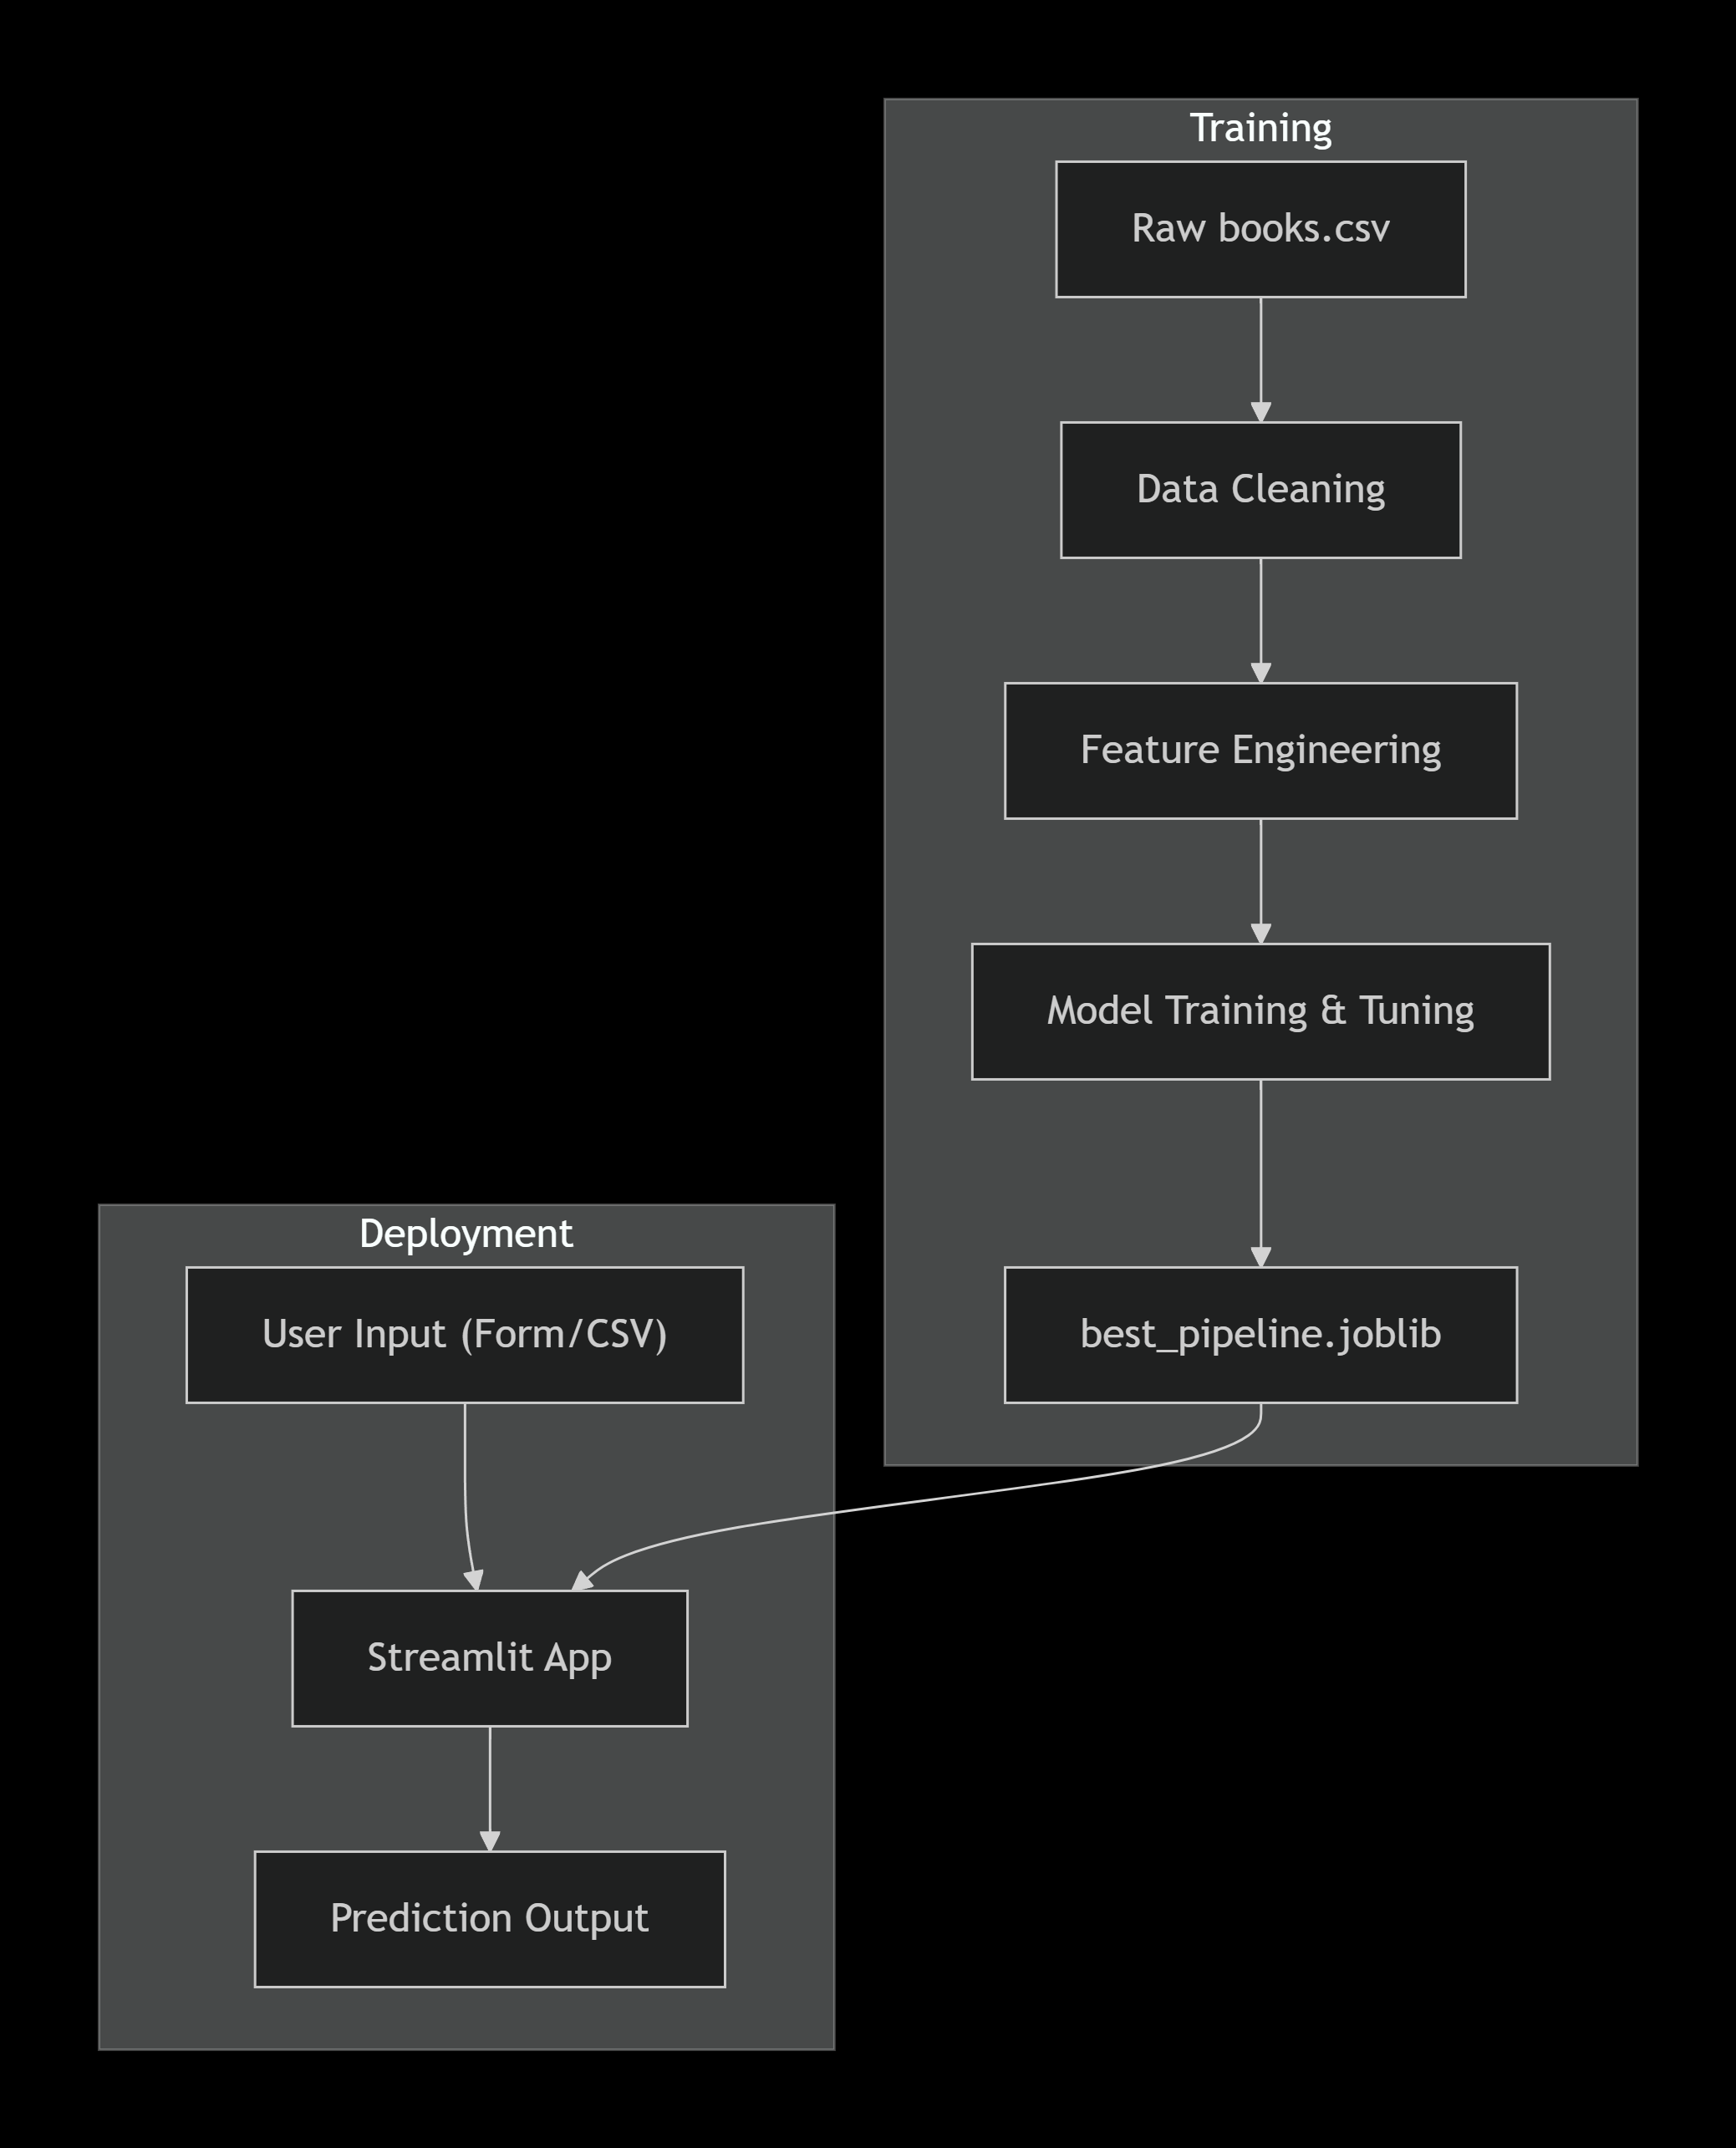
\includegraphics[width=0.85\textwidth]{figures/architecture_diagram.png}
\caption{System architecture: training in Colab, deployment on Windows with Streamlit.}
\label{fig:arch}
\end{figure}

%---------------------------------------------------------------------
\section{Conclusion}
We successfully built a machine learning pipeline that predicts book ratings with a test RMSE of 0.2436 and an R\textsuperscript{2} of 0.3292. The XGBoost model was selected as the final model and was deployed as an interactive Streamlit application.

\subsection{Limitations and Future Work}
\begin{itemize}
    \item \textbf{Target leakage:} \texttt{ratings\_count} and \texttt{text\_reviews\_count} are post‑publication features. For a true cold‑start prediction (before a book gains reviews), these would not be available. A future version could omit these features and rely solely on author/publisher reputation and textual features from the title.
    \item \textbf{Text features:} Only basic title‑derived features were used. Employing TF‑IDF or pre‑trained embeddings on the title (and potentially the book description, if available) could capture genre and style information.
    \item \textbf{Data size:} With only 11K books, more complex models like neural networks or \\ transformer‑based embeddings would likely overfit. Gathering a larger dataset or using data augmentation could improve performance.
    \item \textbf{Hyperparameter tuning:} More exhaustive search (more iterations, wider grids) may yield slight improvements, but the current gains are marginal given the dataset size.
\end{itemize}

The full code, trained model, and instructions are available on GitHub: \url{https://github.com/jettguitteau/book_classification_pythonML}.
The webapp demo video can be seen on Youtube: \url{https://youtu.be/9ORi7gDnzN8}.

\end{document}
